
\label{sec:resultados}

Este capítulo presenta, etapa por etapa, lo que produjo el procedimiento de la Sección~\ref{sec:metodologia}, con los mismos títulos y en el mismo orden. Cada sección abre con la tabla o la figura que sirve de evidencia y la interpreta; los métodos y su sustento no se repiten. Todas las cifras corresponden a la corrida del año 2018 (ventana de enero a diciembre, 23 dominios y 83 municipios objetivo) y se leyeron de las tablas del procesamiento; las comparaciones entre el modelo clásico y el espacial que el procesamiento no guardaba se calcularon a partir de esas tablas, como se indica en la Sección~\ref{sec:res_espacial}. Las tablas largas y las figuras complementarias están en el Apéndice~\ref{app:resultados}; el nombre técnico de cada variable que el texto menciona en lenguaje natural, en el Apéndice~\ref{app:variables}.

%--------------------------------------------------------------------------------------
\section{Obtención de los datos}
\label{sec:res_obtencion}

La Tabla~\ref{tab:res_obtencion} resume lo que quedó cargado en cada capa. De la GEIH se cargaron los cinco módulos del marco antiguo para los doce meses de 2018 y dos meses de 2025 del marco nuevo, que se procesaron para comprobar que la cadena admite ambos marcos pero no entran en la estimación. TerriData llegó con más de 13 millones de registros en formato largo, que en la capa plata se convierten en una fila por entidad, año y mes. El linaje de las tablas, con el cuaderno que escribe cada una, está en el Apéndice~\ref{app:linaje}.

\begin{table}[!htbp]
\centering
\small
\caption{Volumen de datos por fuente y capa. Conteos de 2018 salvo donde se indica. CG: características generales; FT: fuerza de trabajo.}
\label{tab:res_obtencion}
\begin{tabularx}{\linewidth}{>{\raggedright\arraybackslash}p{3.0cm} >{\raggedright\arraybackslash}X >{\raggedleft\arraybackslash}p{3.2cm}}
\toprule
Fuente & Contenido & Registros \\
\midrule
GEIH, capa bronce y plata & Personas en CG & \num{762753} \\
 & FT, ocupados, no ocupados, inactivos & \num{628486}; \num{348015}; \num{42045}; \num{238426} \\
 & Factores de expansión recalculados con el CNPV 2018 & \num{772619} \\
 & Marco nuevo (2025, dos meses; no se usa) & \num{135810} \\
GEIH, capa oro & Tabla de mercado laboral 2018 (personas; viviendas) & \num{762753}; \num{227027} \\
TerriData & Formato largo (bronce) & \num{13147390} \\
 & Formato ancho (plata): filas y columnas & \num{147026} $\times$ \num{1588} \\
Anexo del DANE & Nacional, 25 series de ciudades y anual & 72; \num{1800}; 30 \\
DIVIPOLA & Municipios y áreas no municipalizadas & \num{1122} \\
\bottomrule
\end{tabularx}
\end{table}

%--------------------------------------------------------------------------------------
\section{Limpieza, estandarización y consolidación}
\label{sec:res_limpieza}

Las verificaciones de la etapa 2 se resumen en la Tabla~\ref{tab:res_limpieza}. Ninguna persona quedó sin factor de expansión ni con factor no positivo, y en ningún módulo apareció una llave sin pareja en características generales. Las identidades de la Ecuación~\ref{eq:identidades} se cumplieron en las 288 combinaciones de mes y dominio de 2018, sin ninguna persona clasificada a la vez como ocupada y desocupada. Antes de corregir la lectura de los archivos de enero a marzo, esas mismas identidades fallaban porque toda la población en edad de trabajar quedaba como activa; con la corrección, la bandera de la PEA coincide con la suma de ocupados y desocupados en los doce meses.

\begin{table}[!htbp]
\centering
\small
\caption{Verificaciones de la limpieza y la consolidación, año 2018. OC: ocupados; DS: desocupados; PEI: población económicamente inactiva.}
\label{tab:res_limpieza}
\begin{tabularx}{\linewidth}{>{\raggedright\arraybackslash}X >{\raggedright\arraybackslash}p{5.6cm}}
\toprule
Verificación & Resultado \\
\midrule
Personas sin factor de expansión o con factor $\leq 0$ & 0 de \num{762753} \\
Llaves de FT, ocupados, no ocupados e inactivos sin pareja en CG & 0~\% en cada módulo; sin duplicados \\
Registros de factores sin persona en CG & \num{9866} de \num{772619} (1.28~\%; entre 1.15 y 1.44~\% por mes) \\
PET = PEA + PEI & \num{628486} = \num{390060} + \num{238426}; 0 de 288 combinaciones la rompen \\
PEA = OC + DS & \num{390060} = \num{348015} + \num{42045}; 0 de 288 la rompen \\
Personas ocupadas y desocupadas a la vez & 0 \\
Bandera de la PEA frente a OC + DS, por mes & Coinciden en 12 de 12 meses \\
TerriData: filas antes y después del paso a formato ancho & \num{147026} y \num{147026}; sin llaves duplicadas \\
TerriData: muestra aleatoria y conversión numérica & 10 de 10 coinciden; 261 de \num{10809352} valores (0.002~\%) pasan a nulo \\
\bottomrule
\end{tabularx}
\end{table}

Los \num{9866} registros de factores sin persona en características generales no afectan la estimación: la unión parte de las personas y les agrega su factor, de modo que esos registros quedan fuera. En TerriData, 1,452 de los 1,582 indicadores se clasificaron como numéricos y 130 como cualitativos.

%--------------------------------------------------------------------------------------
\section{Tratamiento de datos faltantes y valores atípicos}
\label{sec:res_faltantes}

Ninguna imputación fue necesaria: ninguna persona quedó sin factor de expansión y las 18 candidatas del catálogo están completas tanto en los dominios como en los 83 municipios objetivo. Los faltantes de TerriData pesan en el pre-filtrado, porque \num{1073} de los \num{1582} indicadores tienen algún vacío en los 23 dominios. Los \num{152314} registros de 2018 sin código de área no se usaron. En las candidatas, la regla del diagrama de caja señaló 22 valores en 13 variables, con Quibdó y Riohacha como los dominios que más se repiten; ninguno se eliminó y la tasa directa no tiene valores señalados. El efecto de cada regla de la Tabla~\ref{tab:met_faltantes} está en la Tabla~\ref{tab:res_faltantes} del Apéndice~\ref{app:resultados}.

%--------------------------------------------------------------------------------------
\section{Definición de los dominios de estimación y correspondencia geográfica}
\label{sec:res_dominios}

La tabla de dominios tiene 52 filas: las 32 capitales y los municipios de las 7 áreas metropolitanas, que suman 27 filas. En 2018 tuvieron muestra 23 dominios, 7 de ellos con área metropolitana, que reúnen 43 municipios (Tabla~\ref{tab:dominios_geih}). La auditoría de los 23 dominios se resume en la Tabla~\ref{tab:res_auditoria}: todos aparecen en el anexo del DANE con el mismo nombre, y la tasa directa de cada uno coincide con la reconstruida del anexo con una diferencia máxima de 0.0005 puntos porcentuales.

\begin{table}[!htbp]
\centering
\small
\caption{Auditoría de la correspondencia geográfica de los 23 dominios (resumen). El detalle por dominio está en el Apéndice~\ref{app:auditoria}.}
\label{tab:res_auditoria}
\begin{tabularx}{\linewidth}{>{\raggedright\arraybackslash}p{4.2cm} >{\raggedright\arraybackslash}X}
\toprule
Campo & Resultado \\
\midrule
Dominios auditados & 23 (16 ciudades y 7 ciudades con A.M.) \\
Nombre en el anexo del DANE & 23 de 23 \\
Geografía de la tasa & Cabeceras de los municipios del dominio (registros con código de área) \\
Geografía de las covariables & Municipio completo (cabecera y resto), TerriData \\
Regla de las covariables & Valor municipal en las 16 ciudades; razón de totales con el denominador propio en las 7 A.M. \\
Tasa directa frente a la del DANE & Diferencia máxima de 0.0005 puntos porcentuales (Ene-Dic 2018) \\
\bottomrule
\end{tabularx}
\end{table}

La auditoría deja a la vista una diferencia de geografía que acompaña todo el trabajo: la tasa de un dominio describe sus cabeceras, mientras que las covariables describen el municipio completo. En los dominios la diferencia es pequeña, porque la población urbana mediana de los 23 es 92.40~\%; en los municipios objetivo, donde el porcentaje urbano es menor, pesa más (Sección~\ref{sec:res_sin_muestra}).

%--------------------------------------------------------------------------------------
\section{Estimación directa de la tasa de desempleo}
\label{sec:res_directa}

La Tabla~\ref{tab:res_directa} presenta la tasa directa de cada dominio con su error estándar, su CV y la cifra del DANE reconstruida para el mismo año. Los 23 dominios quedan como confiables, con CV entre 2.01~\% (Medellín A.M.) y 3.23~\% (Pasto). Las 23 tasas coinciden con las del DANE y la tasa conjunta, ponderada por la PEA expandida, es 10.83~\%, igual al «Total 23 ciudades y A.M.» del año. El error estándar por bootstrap y el de Taylor casi no difieren: su razón tiene mediana 1.000 y va de 0.969 a 1.026.

\begin{table}[!htbp]
\centering
\small
\caption{Estimación directa por dominio, Ene-Dic 2018, personas de 15 años y más. DS: desocupados en la muestra; TD: tasa de desempleo (\%); EE: error estándar en puntos porcentuales, por bootstrap de viviendas (Ecuación~\ref{eq:var_bootstrap}) y por Taylor (Ecuación~\ref{eq:taylor}); CV en \%; TD DANE: reconstruida con los cuatro trimestres del anexo. La PEA y las viviendas de cada dominio están en la Tabla~\ref{tab:dominios_geih}.}
\label{tab:res_directa}
\begin{tabular}{l r r r r r r}
\toprule
Dominio & DS & TD & EE bootstrap & EE Taylor & CV & TD DANE \\
\midrule
Armenia & \num{1996} & 15.49 & 0.34 & 0.34 & 2.21 & 15.49 \\
Barranquilla A.M. & \num{1732} & 8.15 & 0.20 & 0.20 & 2.50 & 8.15 \\
Bogotá & \num{1974} & 10.37 & 0.23 & 0.24 & 2.26 & 10.37 \\
Bucaramanga A.M. & \num{1204} & 8.74 & 0.28 & 0.27 & 3.16 & 8.74 \\
Cali A.M. & \num{1808} & 11.65 & 0.28 & 0.28 & 2.44 & 11.65 \\
Cartagena & \num{1146} & 8.35 & 0.26 & 0.26 & 3.13 & 8.35 \\
Cúcuta A.M. & \num{1875} & 15.98 & 0.37 & 0.37 & 2.29 & 15.98 \\
Florencia & \num{1321} & 12.94 & 0.37 & 0.36 & 2.87 & 12.94 \\
Ibagué & \num{1788} & 13.99 & 0.33 & 0.33 & 2.35 & 13.99 \\
Manizales A.M. & \num{1467} & 11.24 & 0.28 & 0.28 & 2.53 & 11.24 \\
Medellín A.M. & \num{2548} & 11.84 & 0.24 & 0.23 & 2.01 & 11.84 \\
Montería & \num{1393} & 9.47 & 0.27 & 0.27 & 2.80 & 9.47 \\
Neiva & \num{1480} & 11.53 & 0.31 & 0.31 & 2.69 & 11.53 \\
Pasto & \num{1062} & 8.82 & 0.28 & 0.28 & 3.23 & 8.82 \\
Pereira A.M. & \num{1175} & 8.87 & 0.27 & 0.27 & 3.03 & 8.87 \\
Popayán & \num{1403} & 10.68 & 0.30 & 0.30 & 2.77 & 10.68 \\
Quibdó & \num{1616} & 17.81 & 0.44 & 0.44 & 2.47 & 17.81 \\
Riohacha & \num{1957} & 13.88 & 0.32 & 0.33 & 2.32 & 13.88 \\
Santa Marta & \num{1249} & 8.32 & 0.23 & 0.24 & 2.80 & 8.32 \\
Sincelejo & \num{1558} & 9.61 & 0.25 & 0.25 & 2.62 & 9.61 \\
Tunja & \num{1121} & 11.31 & 0.33 & 0.34 & 2.88 & 11.31 \\
Valledupar & \num{1874} & 14.45 & 0.33 & 0.34 & 2.28 & 14.45 \\
Villavicencio & \num{1448} & 11.87 & 0.32 & 0.32 & 2.69 & 11.87 \\
\midrule
Total & \num{36195} & 10.83 & & & & 10.83 \\
\bottomrule
\end{tabular}
\end{table}

La Tabla~\ref{tab:res_ventana} compara las tres ventanas que cierran en diciembre de 2018. Con un mes, ningún dominio alcanza el 5~\% de CV; con el trimestre, 7 de 23; con el año, los 23. El error estándar del mes es 3.62 veces el del año y el del trimestre, 2.00 veces, cerca de lo que se espera por el tamaño de muestra (3.53 y 2.02). Las tasas de las tres ventanas no son iguales: entre el trimestre y el año la correlación entre dominios es 0.95 y la diferencia media es 0.78 puntos porcentuales, con un máximo de 2.05. Esa diferencia es estacional y no un error: el año promedia doce meses y el trimestre, solo el último. La Figura~\ref{fig:res_ventana} muestra los intervalos de cada dominio en las tres ventanas.

\begin{table}[!htbp]
\centering
\small
\caption{Sensibilidad de la estimación directa a la ventana temporal, 23 dominios, cierre en diciembre de 2018. CV en \%; EE en puntos porcentuales. El DANE no publica la tasa mensual por ciudad.}
\label{tab:res_ventana}
\begin{adjustbox}{max width=\linewidth}
\begin{tabular}{l r r r}
\toprule
 & Mes (Dic) & Trimestre (Oct-Dic) & Año (Ene-Dic) \\
\midrule
PEA en la muestra: mínimo y mediana & 681; \num{1039} & \num{2156}; \num{3218} & \num{8997}; \num{12968} \\
Desocupados en la muestra: mínimo & 83 & 215 & \num{1062} \\
EE mediano & 1.03 & 0.57 & 0.28 \\
CV mediano y máximo & 9.26; 11.76 & 5.37; 6.80 & 2.62; 3.23 \\
Confiables / aceptables / no confiables & 0 / 23 / 0 & 7 / 16 / 0 & 23 / 0 / 0 \\
Dominios que coinciden con el DANE & no aplica & 23 de 23 & 23 de 23 \\
Tasa conjunta y cifra del DANE & 10.78; no publicada & 10.33; 10.33 & 10.83; 10.83 \\
\bottomrule
\end{tabular}
\end{adjustbox}
\end{table}

\begin{figure}[!htbp]
\centering
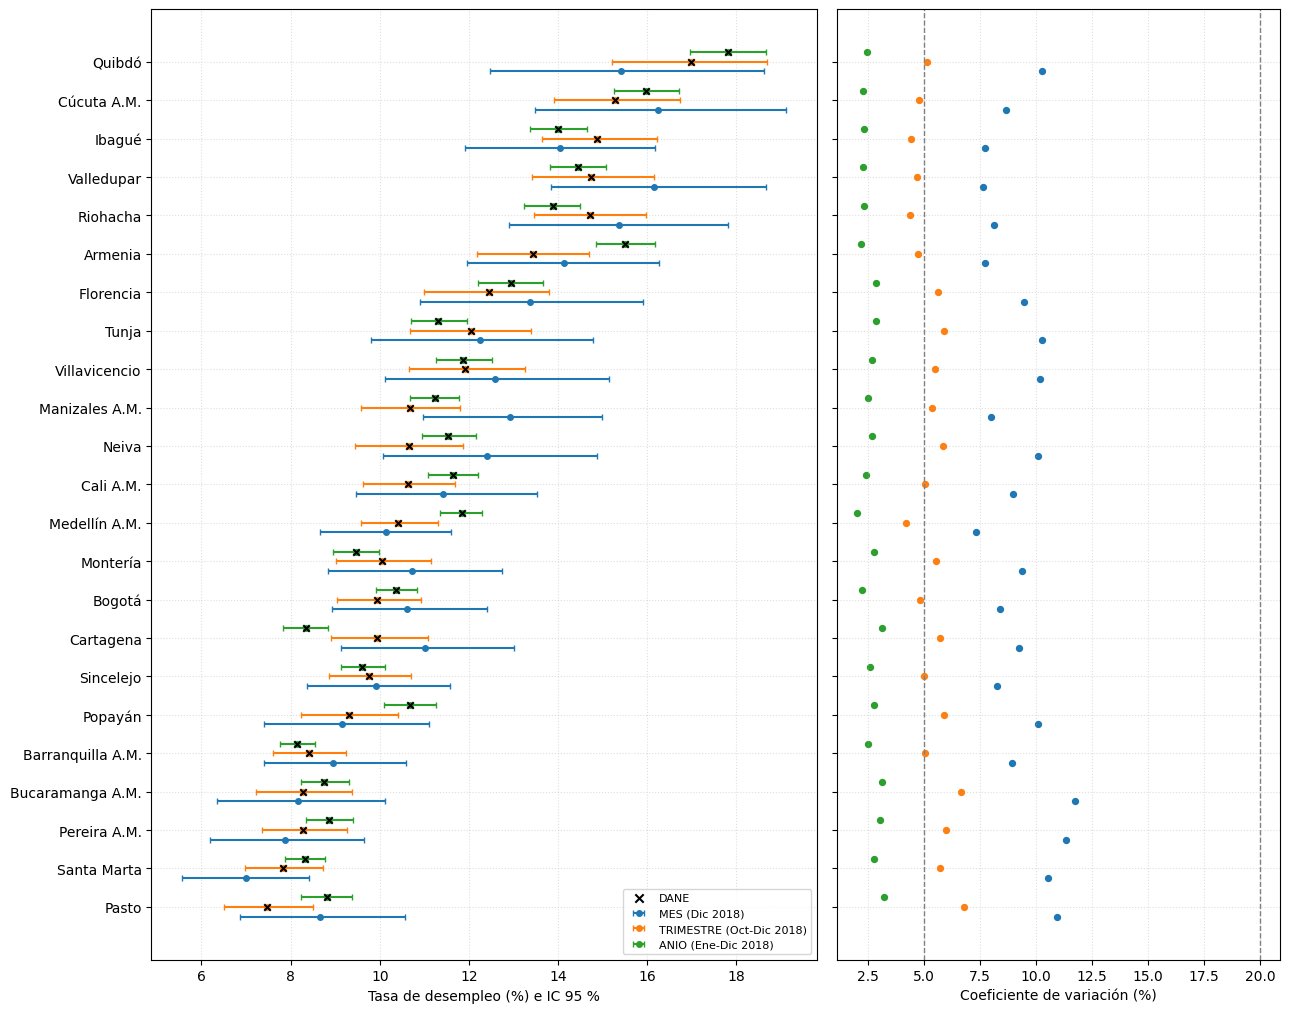
\includegraphics[width=\linewidth]{img/res_ventana_sensibilidad.png}
\caption{Tasa directa e intervalo bootstrap del 95~\% de cada dominio con las ventanas de un mes, un trimestre y un año, todas con cierre en diciembre de 2018. Fuente: tabla de sensibilidad de la ventana temporal.}
\label{fig:res_ventana}
\end{figure}

%--------------------------------------------------------------------------------------
\section{Construcción y agregación de las covariables}
\label{sec:res_covariables}

Las 18 covariables activas tienen dato en diciembre de 2018 para todos los municipios miembro de los dominios y para los 83 municipios objetivo; su geografía, período, unidad y denominador están en la Tabla~\ref{tab:covariables_datos}, y el catálogo con códigos y referencias, en el Apéndice~\ref{app:catalogo}. Las 6 variables de la literatura que no entraron se listan con su motivo en la Tabla~\ref{tab:res_excluidas} del Apéndice~\ref{app:resultados}: cuatro no tienen dato municipal para 2018, la pobreza monetaria no existe en los municipios objetivo y el índice de incidencia del conflicto armado se retiró.

La Tabla~\ref{tab:res_agregacion_am} del Apéndice~\ref{app:resultados} muestra cuánto cambian las covariables de los 7 dominios con área metropolitana si todas se agregan con la población de 15 años y más en lugar de su denominador propio (Ecuación~\ref{eq:agregacion}). En 14 de las 18 el cambio máximo es menor que 1~\%. Cambian mucho la densidad de población, que con la superficie como peso baja hasta 67.67~\% en Bucaramanga A.M., y las tres participaciones del valor agregado, que con el valor agregado como peso cambian hasta 43.94~\% en Cali A.M. En esas variables la regla elegida sí define el valor del dominio.

La tabla de municipios objetivo quedó con 83 filas: 41 del Cauca y 42 del Valle del Cauca. Se excluyó Popayán, que es un dominio por sí solo. Cali y Yumbo se conservaron con Cali A.M. como dominio de referencia.

%--------------------------------------------------------------------------------------
\section{Pre-filtrado de covariables}
\label{sec:res_prefiltrado}

La Tabla~\ref{tab:res_prefiltrado} muestra la cascada. La completitud retira dos de cada tres indicadores; la variabilidad, solo 12 más. El número de sobrevivientes cambia poco con los umbrales: con un CV mínimo entre 0.0001 y 0.01 y una proporción modal entre 0.80 y 0.95 quedan entre 493 y 499; solo con un CV mínimo de 0.05 baja a 475-478. Las 18 candidatas del catálogo pasaron los dos filtros. Entre los 497 sobrevivientes hay 19 grupos de indicadores prácticamente idénticos ($|r| \geq 0.999$), con 140 variables sobrantes, casi todos conteos de población por edad y sexo; se reportaron y no se usaron para decidir.

\begin{table}[!htbp]
\centering
\small
\caption{Cascada del pre-filtrado de los indicadores de TerriData en los 23 dominios.}
\label{tab:res_prefiltrado}
\begin{adjustbox}{max width=\linewidth}
\begin{tabular}{l l r r}
\toprule
Paso & Criterio & Indicadores & Retención (\%) \\
\midrule
Conjunto inicial & Indicadores en formato ancho & \num{1582} & 100.00 \\
Completitud & Sin faltantes en los 23 dominios & 509 & 32.17 \\
Variabilidad & CV $\geq 0.001$ y proporción modal $\leq 0.90$ & 497 & 31.42 \\
\bottomrule
\end{tabular}
\end{adjustbox}
\end{table}

%--------------------------------------------------------------------------------------
\section{Análisis descriptivo}
\label{sec:res_descriptivo}

La Figura~\ref{fig:res_respuesta} resume la tasa directa y su precisión. La tasa va de 8.15~\% en Barranquilla A.M. a 17.81~\% en Quibdó, con media 11.54~\% y mediana 11.31~\%; la asimetría es 0.67 y ningún dominio queda por fuera de la regla del diagrama de caja. El error estándar crece con la tasa (correlación de 0.86): los dominios con más desempleo son también los menos precisos. Quibdó, Cúcuta A.M. y Armenia tienen las tasas más altas; Barranquilla A.M., Santa Marta y Cartagena, las más bajas.

\begin{figure}[!htbp]
\centering
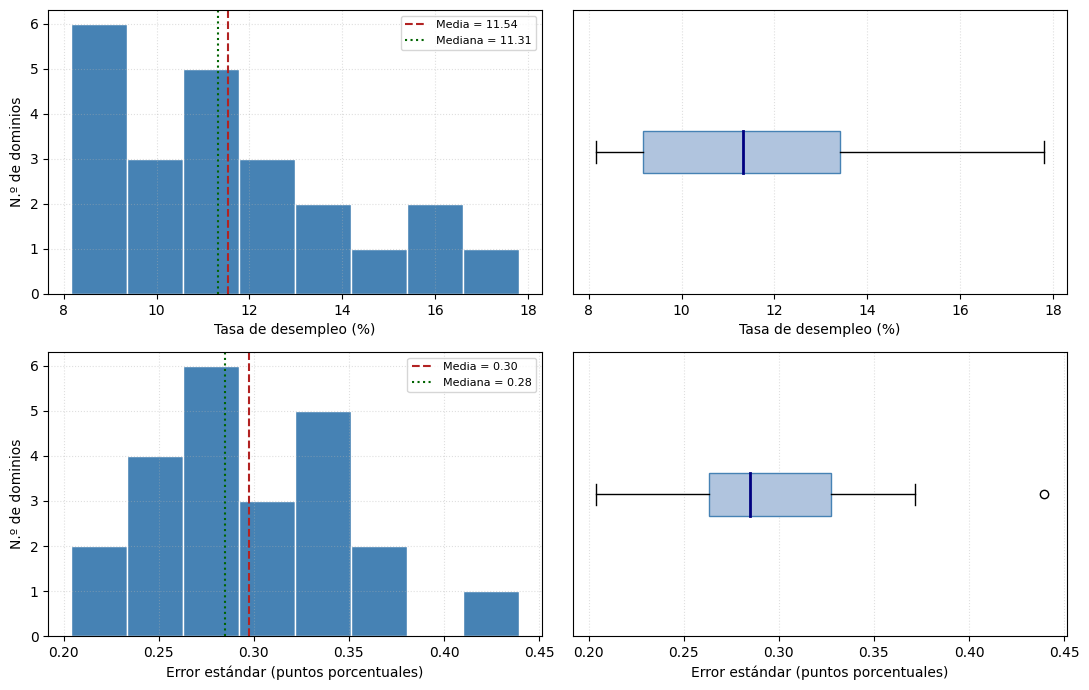
\includegraphics[width=\linewidth]{img/desc_respuesta_precision.png}
\caption{Distribución de la tasa directa, de su error estándar y de su CV en los 23 dominios, y relación entre la tasa y su error estándar. Fuente: tabla de estimación directa.}
\label{fig:res_respuesta}
\end{figure}

La Tabla~\ref{tab:res_bivariado} reúne la descripción bivariada de las 18 candidatas. Ninguna alcanza $|r| \geq 0.50$ con la tasa; diez quedan entre 0.30 y 0.50. En cinco la correlación de Pearson y la de Spearman difieren en más de 0.20, señal de que unos pocos dominios extremos sostienen la relación lineal: la tasa de homicidios, la cobertura de acueducto, el índice de pobreza multidimensional y los dos puntajes de las pruebas Saber 11. Dos candidatas tienen un signo contrario al esperado por el catálogo: la tasa de tránsito a la educación superior y el porcentaje de población urbana.

\begin{table}[!htbp]
\centering
\small
\caption{Asociación de cada candidata con la tasa directa en los 23 dominios. $r$: Pearson; $\rho_S$: Spearman; IC: intervalo de Fisher del 95~\% de $r$ (Ecuación~\ref{eq:ic_fisher}); Signo: esperado por el catálogo. Ordenadas por $|r|$.}
\label{tab:res_bivariado}
\begin{adjustbox}{max width=\linewidth}
\begin{tabular}{l c r r c}
\toprule
Covariable & Signo & $r$ & $\rho_S$ & IC de $r$ \\
\midrule
Tasa de homicidios & $+$ & 0.519 & 0.393 & [0.135, 0.767] \\
Cobertura de acueducto & $-$ & $-0.489$ & $-0.176$ & [$-0.750$, $-0.096$] \\
Cobertura neta en educación media & $-$ & $-0.476$ & $-0.513$ & [$-0.742$, $-0.079$] \\
Índice de pobreza multidimensional & $+$ & 0.441 & 0.184 & [0.035, 0.722] \\
Valor agregado de actividades primarias & $\pm$ & 0.432 & 0.499 & [0.024, 0.717] \\
Ingresos tributarios per cápita & $-$ & $-0.421$ & $-0.489$ & [$-0.710$, $-0.011$] \\
Cobertura neta en educación secundaria & $-$ & $-0.372$ & $-0.393$ & [$-0.680$, 0.047] \\
Valor agregado de actividades secundarias & $\pm$ & $-0.367$ & $-0.286$ & [$-0.677$, 0.053] \\
Valor agregado per cápita & $-$ & $-0.364$ & $-0.385$ & [$-0.675$, 0.056] \\
Tránsito a la educación superior & $-$ & 0.360 & 0.425 & [$-0.061$, 0.673] \\
Índice de desempeño fiscal & $-$ & $-0.315$ & $-0.406$ & [$-0.644$, 0.112] \\
Población joven de 14 a 28 años & $+$ & 0.309 & 0.211 & [$-0.118$, 0.640] \\
Saber 11, lectura crítica & $-$ & $-0.305$ & $-0.085$ & [$-0.637$, 0.122] \\
Densidad de población & $\pm$ & $-0.282$ & $-0.358$ & [$-0.622$, 0.147] \\
Saber 11, matemáticas & $-$ & $-0.269$ & $-0.068$ & [$-0.613$, 0.161] \\
Valor agregado de actividades terciarias & $\pm$ & 0.200 & 0.138 & [$-0.232$, 0.565] \\
Penetración de banda ancha & $-$ & $-0.121$ & $-0.078$ & [$-0.508$, 0.306] \\
Población urbana & $+$ & $-0.017$ & 0.052 & [$-0.426$, 0.398] \\
\bottomrule
\end{tabular}
\end{adjustbox}
\end{table}

En el plano multivariado, seis pares de candidatas tienen $|r| \geq 0.80$: los dos puntajes de Saber 11 (0.970), el valor agregado per cápita y los ingresos tributarios per cápita (0.931), las participaciones secundaria y terciaria del valor agregado ($-0.907$), la lectura crítica y el índice de pobreza multidimensional ($-0.850$), ese índice y la banda ancha ($-0.828$), y el desempeño fiscal y los ingresos tributarios (0.813). La estadística univariada de las candidatas, sus diagramas de caja, los diagramas de dispersión y la matriz de correlaciones están en el Apéndice~\ref{app:descriptivo}.

%--------------------------------------------------------------------------------------
\section{Selección de covariables}
\label{sec:res_seleccion}

La Tabla~\ref{tab:res_seleccion} muestra el recorrido de cada candidata por los cinco pasos. De las 18, tres tienen un valor $q$ de Benjamini-Hochberg menor o igual a 0.10 en el Fay-Herriot univariado, las tres con $q = 0.079$: la tasa de homicidios, la cobertura de acueducto y la cobertura neta en educación media. Con la cota de $\lfloor 23/10 \rfloor = 2$ covariables entraron las dos de mayor $|r_w|$: la tasa de homicidios ($r_w = 0.516$) y la cobertura de acueducto ($r_w = -0.486$). Su VIF es 1.98, por debajo de 5, y exigir el signo esperado no cambia el conjunto.

\begin{table}[!htbp]
\centering
\small
\caption{Ficha de decisión de la selección de covariables. $r_w$: correlación ponderada del Fay-Herriot univariado (Ecuación~\ref{eq:r_ponderada}); $q$: valor de Benjamini-Hochberg sobre 18 (Ecuación~\ref{eq:bh}); Robustez: D = depende de un dominio, E = estable; Soporte: proporción de los 83 municipios objetivo dentro del rango de los dominios. Ordenadas por $|r_w|$.}
\label{tab:res_seleccion}
\begin{adjustbox}{max width=\linewidth}
\begin{tabular}{l r r c r l}
\toprule
Covariable & $r_w$ & $q$ & Robustez & Soporte & Decisión \\
\midrule
Tasa de homicidios & 0.516 & 0.079 & D & 0.747 & Seleccionada \\
Cobertura de acueducto & $-0.486$ & 0.079 & D & 0.867 & Seleccionada \\
Cobertura neta en educación media & $-0.475$ & 0.079 & D & 0.518 & Elegible, fuera de la cota \\
Índice de pobreza multidimensional & 0.438 & 0.101 & D & 0.747 & Redundante (banda ancha) \\
Valor agregado de actividades primarias & 0.431 & 0.101 & E & 0.169 & No elegible \\
Ingresos tributarios per cápita & $-0.420$ & 0.101 & E & 0.590 & Redundante (valor agregado per cápita) \\
Cobertura neta en educación secundaria & $-0.372$ & 0.135 & D & 0.169 & No elegible \\
Valor agregado de actividades secundarias & $-0.365$ & 0.135 & D & 0.663 & Redundante (terciarias) \\
Valor agregado per cápita & $-0.362$ & 0.135 & E & 0.554 & No elegible \\
Tránsito a la educación superior & 0.361 & 0.135 & E & 0.169 & No elegible \\
Índice de desempeño fiscal & $-0.315$ & 0.202 & E & 0.506 & No elegible \\
Población joven de 14 a 28 años & 0.307 & 0.202 & D & 0.723 & No elegible \\
Saber 11, lectura crítica & $-0.302$ & 0.202 & D & 0.699 & Redundante (matemáticas) \\
Densidad de población & $-0.282$ & 0.228 & E & 0.771 & No elegible \\
Saber 11, matemáticas & $-0.266$ & 0.247 & D & 0.771 & No elegible \\
Valor agregado de actividades terciarias & 0.198 & 0.398 & D & 0.373 & No elegible \\
Penetración de banda ancha & $-0.120$ & 0.615 & D & 0.217 & No elegible \\
Población urbana & $-0.017$ & 0.938 & D & 0.265 & No elegible \\
\bottomrule
\end{tabular}
\end{adjustbox}
\end{table}

Los diagnósticos que no deciden dejan advertencias sobre el conjunto elegido. Doce de las 18 candidatas, incluidas las dos seleccionadas, dependen de un dominio según la regla de la Tabla~\ref{tab:met_seleccion}, y en 14 de esos casos el dominio influyente es Quibdó: sin él, la correlación ponderada de la tasa de homicidios baja 0.27 y la de la cobertura de acueducto, 0.39. La Figura~\ref{fig:res_robustez} sitúa cada candidata según su distancia de Cook máxima y ese cambio. En soporte, solo la cobertura de acueducto supera el 0.80; con la tasa de homicidios, 21 de los 83 municipios objetivo quedan fuera del rango de los dominios. La forma lineal resultó adecuada en las tres elegibles (ni el término cuadrático ni el logaritmo mejoran el AIC). El detalle de cada paso está en el Apéndice~\ref{app:seleccion}.

\begin{figure}[!htbp]
\centering
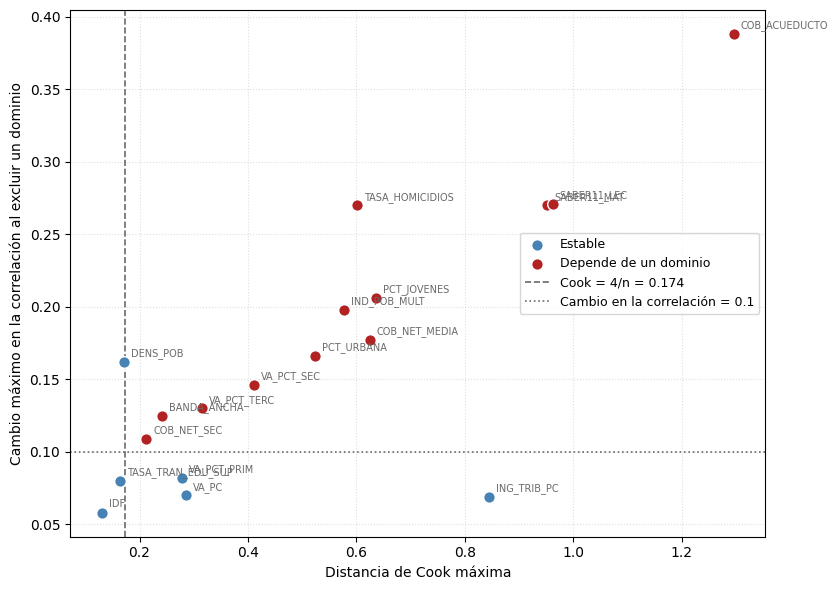
\includegraphics[width=0.85\linewidth]{img/eda_robustez.png}
\caption{Diagnóstico de robustez de las 18 candidatas: distancia de Cook máxima del Fay-Herriot univariado y cambio máximo de $r_w$ al retirar un dominio. Las líneas marcan $4/n = 0.174$ y el cambio de 0.10. Fuente: tabla de diagnósticos de covariables.}
\label{fig:res_robustez}
\end{figure}

%--------------------------------------------------------------------------------------
\section{Ajuste y selección del modelo Fay-Herriot clásico (benchmark)}
\label{sec:res_fh_clasico}

La Tabla~\ref{tab:res_especificaciones} compara las cuatro especificaciones. En EC1, con las dos covariables seleccionadas, ninguna es significativa ($p = 0.190$ y $p = 0.351$): comparten buena parte de la información, porque las dos dependen de Quibdó. Por eso EC1 no compite. Entre las tres que cumplen la regla, EC3 (tasa de homicidios) tiene el menor AIC, 108.904; EC2 (cobertura de acueducto) queda a 0.918 y es equivalente por la regla de $\Delta$AIC $\leq 2$. Como las dos tienen una covariable, la parsimonia no las separa y la elección la define el AIC. EC0 queda a 5.138 del mejor y no es equivalente. El AICc ordena igual. La RMSE de dejar un dominio fuera, que es descriptiva, también ordena a EC3 primero.

\begin{table}[!htbp]
\centering
\small
\caption{Especificaciones candidatas del modelo base Fay-Herriot clásico. $p$: valor $p$ máximo de las covariables; $\hat{\sigma}_u^2$ en puntos porcentuales al cuadrado; AIC y AICc con la verosimilitud ML (Ecuación~\ref{eq:aic}); RMSE: error de estimación de cada dominio retirado, con las covariables fijas (descriptiva). La especificación elegida está marcada con *.}
\label{tab:res_especificaciones}
\begin{adjustbox}{max width=\linewidth}
\begin{tabular}{l l r r r r r r r}
\toprule
 & Covariables & $p$ & $\hat{\sigma}_u^2$ & $R^2$ & AIC & $\Delta$AIC & AICc & RMSE \\
\midrule
EC3* & Homicidios & 0.006 & 5.529 & 0.269 & 108.904 & 0.000 & 110.167 & 2.52 \\
EC2 & Acueducto & 0.011 & 5.757 & 0.239 & 109.822 & 0.918 & 111.085 & 2.60 \\
EC1 & Homicidios y acueducto & 0.351 & 5.564 & 0.299 & 109.926 & 1.023 & 112.148 & 2.55 \\
EC0 & Solo intercepto & no aplica & 7.209 & 0.000 & 114.042 & 5.138 & 114.642 & 2.77 \\
\bottomrule
\end{tabular}
\end{adjustbox}
\end{table}

La Tabla~\ref{tab:res_coeficientes} muestra los coeficientes del benchmark. Cada 10 homicidios adicionales por cada 100,000 habitantes se asocian con 0.99 puntos porcentuales más de tasa de desempleo, condicional a la selección. El $R^2$ del componente sintético es 0.269: la tasa de homicidios deja sin explicar la mayor parte de la diferencia entre dominios. Frente al modelo de solo intercepto, $\hat{\sigma}_u^2$ baja de 7.209 a 5.529, es decir, un 23~\%.

\begin{table}[!htbp]
\centering
\small
\caption{Coeficientes del benchmark EC3, estimados por GLS (Ecuación~\ref{eq:gls}) con $\hat{\sigma}_u^2 = 5.529$ por REML. EE: error estándar. Los valores $p$ son descriptivos (Sección~\ref{sec:met_fh_clasico}).}
\label{tab:res_coeficientes}
\begin{tabular}{l r r r r}
\toprule
Parámetro & $\hat{\beta}$ & EE & $z$ & $p$ \\
\midrule
Intercepto & 9.191 & 0.979 & 9.388 & $<0.001$ \\
Tasa de homicidios (por 100,000 habitantes) & 0.099 & 0.036 & 2.761 & 0.006 \\
\bottomrule
\end{tabular}
\end{table}

Con varianzas de muestreo entre 0.04 y 0.19 frente a $\hat{\sigma}_u^2 = 5.529$, el peso de la estimación directa es alto en todos los dominios: $\hat{\gamma}_d$ va de 0.966 en Quibdó a 0.993 en Barranquilla A.M., con media 0.984. En consecuencia, el EBLUP casi coincide con la estimación directa (la mayor diferencia es $-0.10$ puntos porcentuales, en Cúcuta A.M.) y el ECM baja en promedio un 1.16~\% frente a $\psi_d$. Los 23 dominios siguen siendo confiables con el EBLUP (Figura~\ref{fig:res_cv}). La tabla de los 23 EBLUP con su ECM y su CV está en el Apéndice~\ref{app:dominios_modelo}.

\begin{figure}[!htbp]
\centering
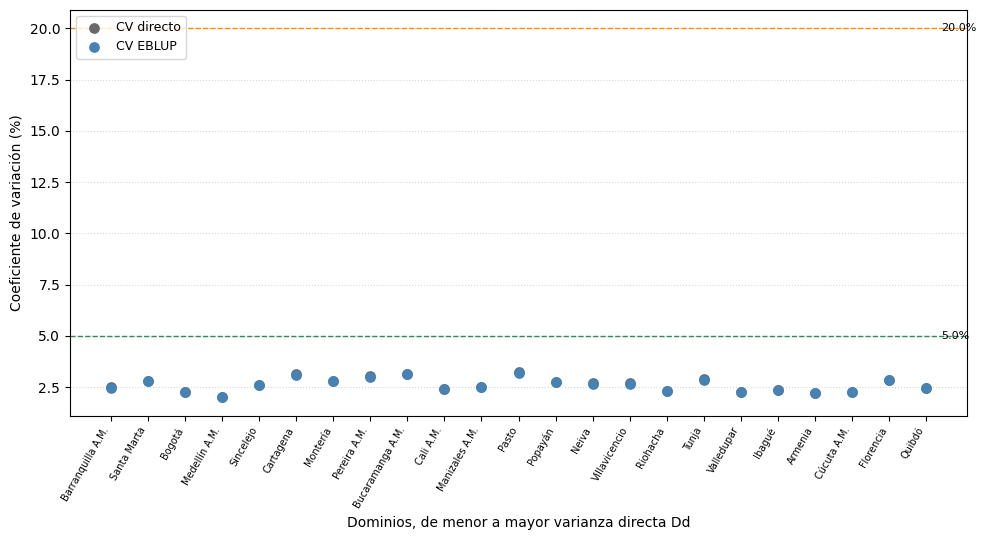
\includegraphics[width=0.85\linewidth]{img/fh_ganador_cv.png}
\caption{CV de la estimación directa y del EBLUP del benchmark por dominio, ordenados por la varianza de muestreo. Fuente: tabla de resultados del Fay-Herriot clásico.}
\label{fig:res_cv}
\end{figure}

%--------------------------------------------------------------------------------------
\section{Validación de supuestos y sensibilidad del benchmark}
\label{sec:res_supuestos}

La Tabla~\ref{tab:res_diagnosticos} reúne los diagnósticos del benchmark con el formato de la nota metodológica del DANE \cite{DANE_SAE_2025}. Los diagnósticos no muestran evidencia fuerte contra la aproximación normal en el benchmark, dentro de la limitada potencia disponible con 23 áreas. La media de los residuos es cercana a cero por construcción y no informa sobre sesgo. Los residuos tampoco muestran dependencia espacial con ninguna de las cuatro matrices (Sección~\ref{sec:res_espacial}). Los histogramas y gráficos de contracción de las cuatro especificaciones están en el Apéndice~\ref{app:especificaciones}.

\begin{table}[!htbp]
\centering
\small
\caption{Diagnósticos del benchmark EC3 sobre los residuos estandarizados (Ecuación~\ref{eq:residuos}).}
\label{tab:res_diagnosticos}
\begin{tabularx}{\linewidth}{>{\raggedright\arraybackslash}p{2.8cm} >{\raggedright\arraybackslash}p{3.9cm} >{\raggedright\arraybackslash}p{2.6cm} >{\raggedright\arraybackslash}X}
\toprule
Supuesto & Medida & Valor & Lectura \\
\midrule
Normalidad & Shapiro-Wilk (Ecuación~\ref{eq:shapiro}) & $W = 0.954$; $p = 0.357$ & Sin evidencia fuerte en contra, con baja potencia \\
Media cero & Media de los residuos & 0.002 & Cercana a cero por construcción del GLS \\
Varianza & Desviación estándar & 0.977 & Cercana a 1: $\psi_d$ y $\hat{\sigma}_u^2$ son compatibles con la dispersión observada \\
Independencia espacial & I de Moran, 3 vecinos (Ecuación~\ref{eq:moran}) & $I = 0.093$; $p = 0.333$ & Sin autocorrelación detectable \\
Influencia & Cook máxima (Ecuación~\ref{eq:cook}) & 0.601 (Quibdó) & Quibdó y Cali A.M. superan $4/n = 0.174$ \\
\bottomrule
\end{tabularx}
\end{table}

La Tabla~\ref{tab:res_estabilidad} resume la estabilidad del coeficiente de la tasa de homicidios. Al retirar un dominio, $\hat{\beta}_1$ queda entre 0.061 (sin Quibdó) y 0.125 (sin Cali A.M.). Sin Quibdó el cambio es de $-38.2$~\%, equivale a 1.05 errores estándar, supera el umbral de 1 y el coeficiente deja de ser significativo ($p = 0.256$); es el único de los 23 reajustes que cruza el umbral de significancia y ninguno cambia el signo. En el bootstrap de dominios el intervalo del 95~\% va de 0.011 a 0.191, el signo se conserva en el 98.6~\% de las réplicas y la significancia, en el 70.4~\%. La Figura~\ref{fig:res_loao} muestra el cambio estandarizado por dominio.

\begin{table}[!htbp]
\centering
\small
\caption{Estabilidad del coeficiente de la tasa de homicidios: 23 reajustes dejando un dominio fuera (reestimando $\hat{\sigma}_u^2$) y \num{1000} réplicas bootstrap de dominios. Cambio en EE: Ecuación~\ref{eq:dfbeta}.}
\label{tab:res_estabilidad}
\begin{tabularx}{\linewidth}{>{\raggedright\arraybackslash}X >{\raggedright\arraybackslash}p{6.4cm}}
\toprule
Medida & Resultado \\
\midrule
$\hat{\beta}_1$ con los 23 dominios & 0.099 (EE 0.036) \\
Mínimo y máximo al retirar un dominio & 0.061 (sin Quibdó) y 0.125 (sin Cali A.M.) \\
Cambio máximo & $-38.2$~\% $= -1.05$ EE (Quibdó); siguientes: Cali A.M. ($+0.71$ EE) y Tunja ($+0.25$ EE) \\
Cambios de signo y de significancia & 0 de 23 y 1 de 23 (Quibdó, $p = 0.256$) \\
Bootstrap: intervalo del 95~\% & [0.011, 0.191] \\
Bootstrap: mismo signo y $p < 0.05$ & 98.6~\% y 70.4~\% de las réplicas \\
Mayor cambio de un EBLUP de los otros dominios & 0.05 puntos porcentuales \\
Mayor cambio de una estimación municipal & $-7.65$ puntos porcentuales (Corinto, sin Quibdó) \\
Cambio máximo de $\hat{\sigma}_u^2$ & 11~\% \\
\bottomrule
\end{tabularx}
\end{table}

\begin{figure}[!htbp]
\centering
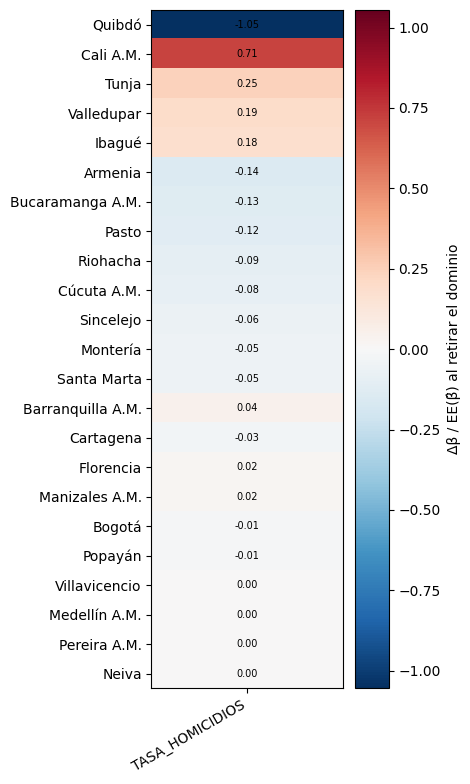
\includegraphics[width=0.85\linewidth]{img/fh_loao_influencia.png}
\caption{Cambio de cada coeficiente del benchmark, en errores estándar, al retirar cada dominio. Fuente: tabla de influencia dejar-un-dominio-fuera del Fay-Herriot clásico.}
\label{fig:res_loao}
\end{figure}

Los EBLUP de los dominios casi no se mueven al retirar un dominio, porque cada uno se apoya en su propia estimación directa. Las estimaciones municipales sí: retirar Quibdó cambia más de 0.5 puntos porcentuales la estimación de 51 municipios y retirar Cali A.M., la de 45. La influencia de un solo dominio se transmite a los municipios a través del coeficiente.

La Tabla~\ref{tab:res_varianza} resume la sensibilidad a la varianza de muestreo. Las varianzas alternativas son parecidas a la base: la de Taylor tiene razón mediana 1.000 con la del bootstrap, y la del bootstrap por personas es menor (razón 1.104, entre 0.939 y 1.173), como se espera al ignorar la correlación dentro de la vivienda. Las dos GVF se ajustan bien ($R^2$ de 0.970 y 0.976; Figura~\ref{fig:app_gvf}). En los nueve escenarios el benchmark sigue siendo EC3, el coeficiente conserva signo y significancia, y el EBLUP cambia como máximo 0.20 puntos porcentuales. Solo al triplicar $\psi_d$ cuatro dominios pasan de confiables a aceptables. La razón $\hat{\sigma}_u^2/\bar{\psi}$, entre 19.5 y 184.2, explica por qué el modelo es poco sensible a $\psi_d$: con una varianza entre dominios tan grande frente a la de muestreo, $\hat{\gamma}_d$ se mantiene cerca de 1 en todos los escenarios \cite[p.~143]{Benedetti2024}.

\begin{table}[!htbp]
\centering
\small
\caption{Escenarios de la varianza de muestreo. $\bar{\psi}$: media de $\psi_d$; $\Delta$EBLUP y $\Delta$sintético: cambio máximo frente al escenario base, en puntos porcentuales; Conf.: dominios confiables con el EBLUP. En todos los escenarios el benchmark es EC3.}
\label{tab:res_varianza}
\begin{adjustbox}{max width=\linewidth}
\begin{tabular}{l r r r r r r}
\toprule
Escenario & $\hat{\sigma}_u^2$ & $\hat{\sigma}_u^2/\bar{\psi}$ & $\min \hat{\gamma}_d$ & $\Delta$EBLUP & $\Delta$sintético & Conf. \\
\midrule
Base (bootstrap de viviendas) & 5.529 & 60.7 & 0.966 & 0.00 & 0.00 & 23 \\
Taylor & 5.527 & 60.4 & 0.966 & 0.00 & 0.00 & 23 \\
GVF A & 5.524 & 60.6 & 0.967 & 0.01 & 0.00 & 23 \\
$\psi_d \times 1/3$ & 5.595 & 184.2 & 0.989 & 0.07 & 0.04 & 23 \\
$\psi_d \times 1/2$ & 5.578 & 122.4 & 0.983 & 0.05 & 0.03 & 23 \\
$\psi_d \times 2/3$ & 5.562 & 91.6 & 0.977 & 0.03 & 0.02 & 23 \\
$\psi_d \times 3/2$ & 5.480 & 40.1 & 0.950 & 0.05 & 0.03 & 23 \\
$\psi_d \times 2$ & 5.430 & 29.8 & 0.934 & 0.10 & 0.06 & 23 \\
$\psi_d \times 3$ & 5.332 & 19.5 & 0.902 & 0.20 & 0.13 & 19 \\
\bottomrule
\end{tabular}
\end{adjustbox}
\end{table}

%--------------------------------------------------------------------------------------
\section{Validación predictiva dejar-un-dominio-fuera}
\label{sec:res_validacion}

Con los 23 dominios, la selección repetida reproduce el conjunto de la etapa 9 y el benchmark de la etapa 10, como exige la verificación de la Tabla~\ref{tab:met_validacion}. La Tabla~\ref{tab:res_validacion} presenta las métricas de los dos ejercicios y del modelo de solo intercepto.

\begin{table}[!htbp]
\centering
\small
\caption{Validación predictiva dejar-un-dominio-fuera: error de la estimación sintética de cada dominio retirado frente a su estimación directa (Ecuación~\ref{eq:metricas_val}). Errores en puntos porcentuales; cobertura del intervalo nominal del 95~\%; habilidad frente al modelo de solo intercepto.}
\label{tab:res_validacion}
\begin{adjustbox}{max width=\linewidth}
\begin{tabular}{l r r r}
\toprule
Métrica & Covariables fijas & Procedimiento completo & Solo intercepto \\
\midrule
RMSE & 2.52 & 3.43 & 2.77 \\
MAE & 2.13 & 2.91 & 2.23 \\
Sesgo medio & $-0.07$ & $-0.41$ & $-0.01$ \\
RMSE corregida por ruido & 2.51 & 3.42 & 2.76 \\
$Z_{\text{pred}}$: media y desviación & $-0.02$; 1.05 & $-0.17$; 1.44 & $-0.02$; 1.07 \\
Cobertura (\%) & 100.00 & 86.96 & 95.65 \\
Habilidad frente al modelo nulo & 0.17 & $-0.54$ & no aplica \\
\bottomrule
\end{tabular}
\end{adjustbox}
\end{table}

Con las covariables fijas, la tasa de homicidios mejora la RMSE del modelo nulo en un 17~\% (2.52 frente a 2.77). Ese ejercicio es optimista, porque la covariable se eligió viendo a todos los dominios. Cuando la selección se repite en cada iteración, la RMSE sube a 3.43, por encima de la del modelo de solo intercepto, y la habilidad pasa a $-0.54$: el procedimiento completo estima peor que el promedio de los dominios. La diferencia entre 2.52 y 3.43 es el costo de seleccionar y estimar con los mismos 23 dominios. Frente al error dentro de muestra (2.27), la validación con covariables fijas lo infla 1.11 veces y el procedimiento completo, 1.52.

La inestabilidad de la selección explica ese costo. El procedimiento reproduce el benchmark en 14 de las 23 iteraciones y produce 6 conjuntos distintos; la tasa de homicidios entra al benchmark en el 69.57~\% de las iteraciones y la cobertura de acueducto, en el 8.70~\% (Tabla~\ref{tab:res_frecuencia} del Apéndice~\ref{app:resultados}). Sin Florencia, Quibdó, Riohacha o Pasto no queda ninguna covariable elegible y se usa solo el intercepto; sin Bogotá entra el ingreso tributario per cápita, sin Neiva el valor agregado primario y sin Armenia la cobertura neta en media. En tres dominios el error estandarizado supera 1.96 en valor absoluto: Armenia ($-3.17$), Quibdó ($-2.66$) y Cúcuta A.M. ($-2.15$). Los errores por dominio y la figura de los dos ejercicios están en el Apéndice~\ref{app:validacion}.

%--------------------------------------------------------------------------------------
\section{Modelo Fay-Herriot espacial y comparación con el benchmark}
\label{sec:res_espacial}

Los 23 dominios están lejos entre sí: el vecino más cercano de cada uno está entre 30 y 158 km, con mediana de 106 km, y 12 lo tienen a más de 100 km. Los municipios objetivo están más cerca de algún dominio: la distancia mediana al más cercano es 46.3 km en el Cauca y 44.6 km en el Valle del Cauca. La Tabla~\ref{tab:res_espacial} presenta el ajuste del benchmark y de las especificaciones espaciales con la tasa de homicidios fija.

\begin{table}[!htbp]
\centering
\small
\caption{Ajuste del benchmark y de las especificaciones espaciales (misma respuesta, mismos $\psi_d$, mismos 23 dominios, tasa de homicidios fija). $\Delta$AIC = AIC clásico $-$ AIC espacial (positivo favorece al espacial); LRT de $\rho = 0$ (Ecuación~\ref{eq:lrt}); RMSE de la validación dejar-un-dominio-fuera del predictor espacial (estructura completa) o de la estimación sintética (muestra). Las ocho especificaciones están en el Apéndice~\ref{app:espacial}.}
\label{tab:res_espacial}
\begin{adjustbox}{max width=\linewidth}
\begin{tabular}{l r r r r r r r}
\toprule
Especificación & $\hat{\sigma}_u^2$ & $\hat{\rho}$ & AIC & $\Delta$AIC & LRT & $p$ & RMSE \\
\midrule
Clásico (benchmark) & 5.529 & no aplica & 108.904 & no aplica & no aplica & no aplica & 2.52 \\
3 vecinos, muestra & 5.383 & 0.234 & 110.572 & $-1.669$ & 0.331 & 0.565 & 2.53 \\
3 vecinos, completa (referencia) & 4.825 & 0.372 & 109.403 & $-0.500$ & 1.500 & 0.221 & 2.35 \\
Otras seis: mínimo & 5.101 & 0.187 & 110.105 & $-1.998$ & 0.003 & 0.371 & 2.48 \\
Otras seis: máximo & 5.631 & 0.891 & 110.901 & $-1.201$ & 0.799 & 0.960 & 2.86 \\
\bottomrule
\end{tabular}
\end{adjustbox}
\end{table}

Ninguna de las ocho especificaciones espaciales cumple el criterio. En la estructura «muestra» del escenario de referencia, $\hat{\rho} = 0.234$ y $p(\text{LRT}) = 0.565$; en todas, $p \geq 0.221$, y el AIC del espacial es mayor que el del clásico, lo que corresponde a $\text{LRT} < 2$. El perfil de verosimilitud del escenario de referencia es plano: su intervalo del 95~\% para $\rho$ va de $-0.15$ a 0.75 (Figura~\ref{fig:app_perfil_rho}). Los $\hat{\rho}$ de la estructura «completa» llegan hasta 0.891 con distancia inversa de potencia 1, pero cambian según los municipios que se incluyen como nodos (0.398 con solo los del Valle y 0.262 con solo los del Cauca, con 3 vecinos), por lo que no se interpretan. Ubicar el nodo de cada área metropolitana en la media de sus municipios cambia $\hat{\rho}$ como máximo en 0.131 y ningún $p$ baja de 0.354. Con este resultado, el modelo recomendado es el benchmark clásico y el espacial queda como análisis de sensibilidad.

La Tabla~\ref{tab:res_moran} compara el I de Moran de los residuos estandarizados del clásico con el de los residuos del SEBLUP. Ningún índice es significativo; los del clásico van de $-0.023$ a 0.093 y los del espacial, de $-0.115$ a $-0.038$. La tasa directa tampoco muestra autocorrelación (I entre $-0.028$ y 0.003). La Figura~\ref{fig:res_mapa_residuos} muestra los residuos sobre el mapa: los dominios con residuos del mismo signo no se agrupan, y los mayores (Cúcuta A.M. y Valledupar, positivos; Barranquilla A.M. y Cartagena, negativos) quedan en regiones distintas.

\begin{table}[!htbp]
\centering
\small
\caption{I de Moran de los residuos estandarizados del clásico y de los residuos del SEBLUP, con la misma matriz estandarizada por filas en cada escenario; $p$ por \num{9999} permutaciones. $E[I] = -0.045$.}
\label{tab:res_moran}
\begin{tabular}{l r r r r r r}
\toprule
 & \multicolumn{2}{c}{Clásico} & \multicolumn{2}{c}{SEBLUP muestra} & \multicolumn{2}{c}{SEBLUP completa} \\
\cmidrule(lr){2-3}\cmidrule(lr){4-5}\cmidrule(lr){6-7}
Matriz & $I$ & $p$ & $I$ & $p$ & $I$ & $p$ \\
\midrule
3 vecinos & 0.093 & 0.333 & $-0.043$ & 0.984 & $-0.110$ & 0.658 \\
5 vecinos & 0.005 & 0.605 & $-0.038$ & 0.938 & $-0.038$ & 0.936 \\
Inversa, potencia 1 & $-0.023$ & 0.650 & $-0.055$ & 0.848 & $-0.057$ & 0.819 \\
Inversa, potencia 2 & 0.013 & 0.599 & $-0.069$ & 0.830 & $-0.115$ & 0.522 \\
\bottomrule
\end{tabular}
\end{table}

\begin{figure}[!htbp]
\centering
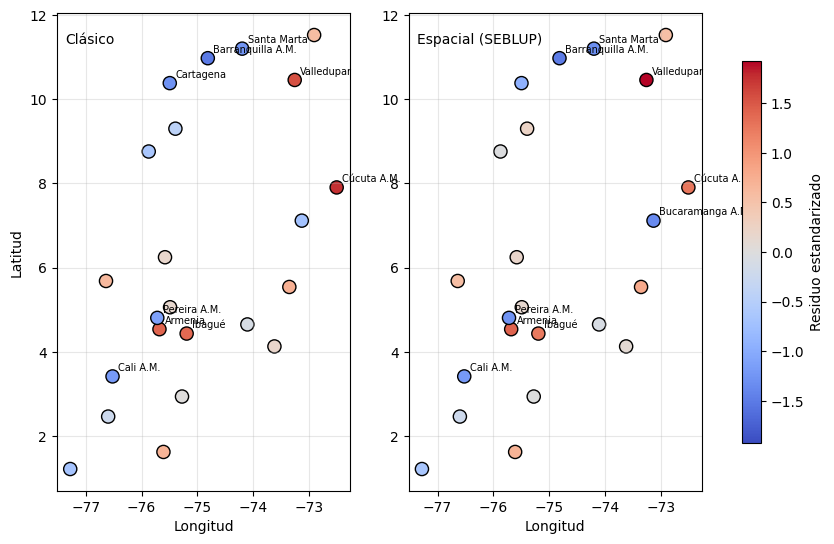
\includegraphics[width=0.9\linewidth]{img/fhe_mapa_residuos.png}
\caption{Residuos estandarizados de los 23 dominios en el clásico y en el SEBLUP del escenario de referencia (3 vecinos, estructura completa), ubicados en la cabecera de la capital. Fuente: tablas de Moran y de comparación del modelo espacial.}
\label{fig:res_mapa_residuos}
\end{figure}

La Tabla~\ref{tab:res_comparacion} completa la comparación controlada con la incertidumbre, las estimaciones y los coeficientes. El ECM y el CV del SEBLUP de los 23 dominios, su peso $\hat{\gamma}^{S}_d$ y las diferencias en los dominios no los guardaba el procesamiento; se calcularon reajustando el SEBLUP del escenario de referencia con la misma clase del código, que reproduce $\hat{\rho} = 0.372$ y $\hat{\sigma}_u^2 = 4.825$ con 500 réplicas válidas de 500 (Ecuaciones~\ref{eq:seblup} y~\ref{eq:gamma_esp}).

\begin{table}[!htbp]
\centering
\small
\caption{Comparación controlada entre el benchmark (EBLUP y estimación sintética) y el escenario espacial de referencia (SEBLUP y predictor espacial). Diferencias = espacial $-$ clásico, en puntos porcentuales; clases de CV con los umbrales de 5 y 20~\%. Fuente: tablas del modelo; dominios: cálculo propio sobre esas tablas.}
\label{tab:res_comparacion}
\begin{tabularx}{\linewidth}{>{\raggedright\arraybackslash}X >{\raggedleft\arraybackslash}p{3.3cm} >{\raggedleft\arraybackslash}p{3.3cm}}
\toprule
Elemento & 23 dominios & 83 municipios \\
\midrule
CV mediano: clásico y espacial (\%) & 2.60 y 2.60 & 19.49 y 19.87 \\
ECM medio: clásico y espacial & 0.090 y 0.091 & no aplica \\
Peso de la directa: $\hat{\gamma}_d$ y $\hat{\gamma}^S_d$ (medias) & 0.984 y 0.982 & no aplica \\
Diferencia media & 0.00 & $-0.03$ \\
Diferencia absoluta media & 0.01 & 0.22 \\
Diferencia absoluta máxima & 0.02 & 2.79 (Cali) \\
Casos con diferencia absoluta mayor que 0.5 & 0 & 8 \\
Correlación de Pearson y de Spearman & 1.000 y 1.000 & 0.992 y 0.987 \\
Cambios de clase de confiabilidad & 0 & 8 (7 de no confiable a aceptable) \\
Coeficiente de la tasa de homicidios (EE) & \multicolumn{2}{c}{clásico 0.099 (0.036); espacial 0.102 (0.035); diferencia 0.07 EE} \\
\bottomrule
\end{tabularx}
\end{table}

En los dominios, las dos estimaciones son prácticamente iguales: la mayor diferencia es 0.02 puntos porcentuales y la precisión no cambia. En los municipios, la estimación espacial agrega a la sintética el efecto que el modelo infiere de los dominios cercanos; ese efecto es pequeño en casi todos (Figura~\ref{fig:res_espacial_estimaciones}). Las dos diferencias grandes son Cali y Yumbo ($-2.79$ y $-2.72$ puntos porcentuales), que reciben el efecto estimado de Cali A.M. y no uno propio. Les siguen Caicedonia (0.79), Jamundí ($-0.74$), Ulloa (0.66), El Águila (0.64), Alcalá (0.59) y Candelaria ($-0.55$), todos a menos de 40 km de un dominio. El coeficiente de la tasa de homicidios cambia menos de 0.13 errores estándar del clásico en las ocho especificaciones.

\begin{figure}[!htbp]
\centering
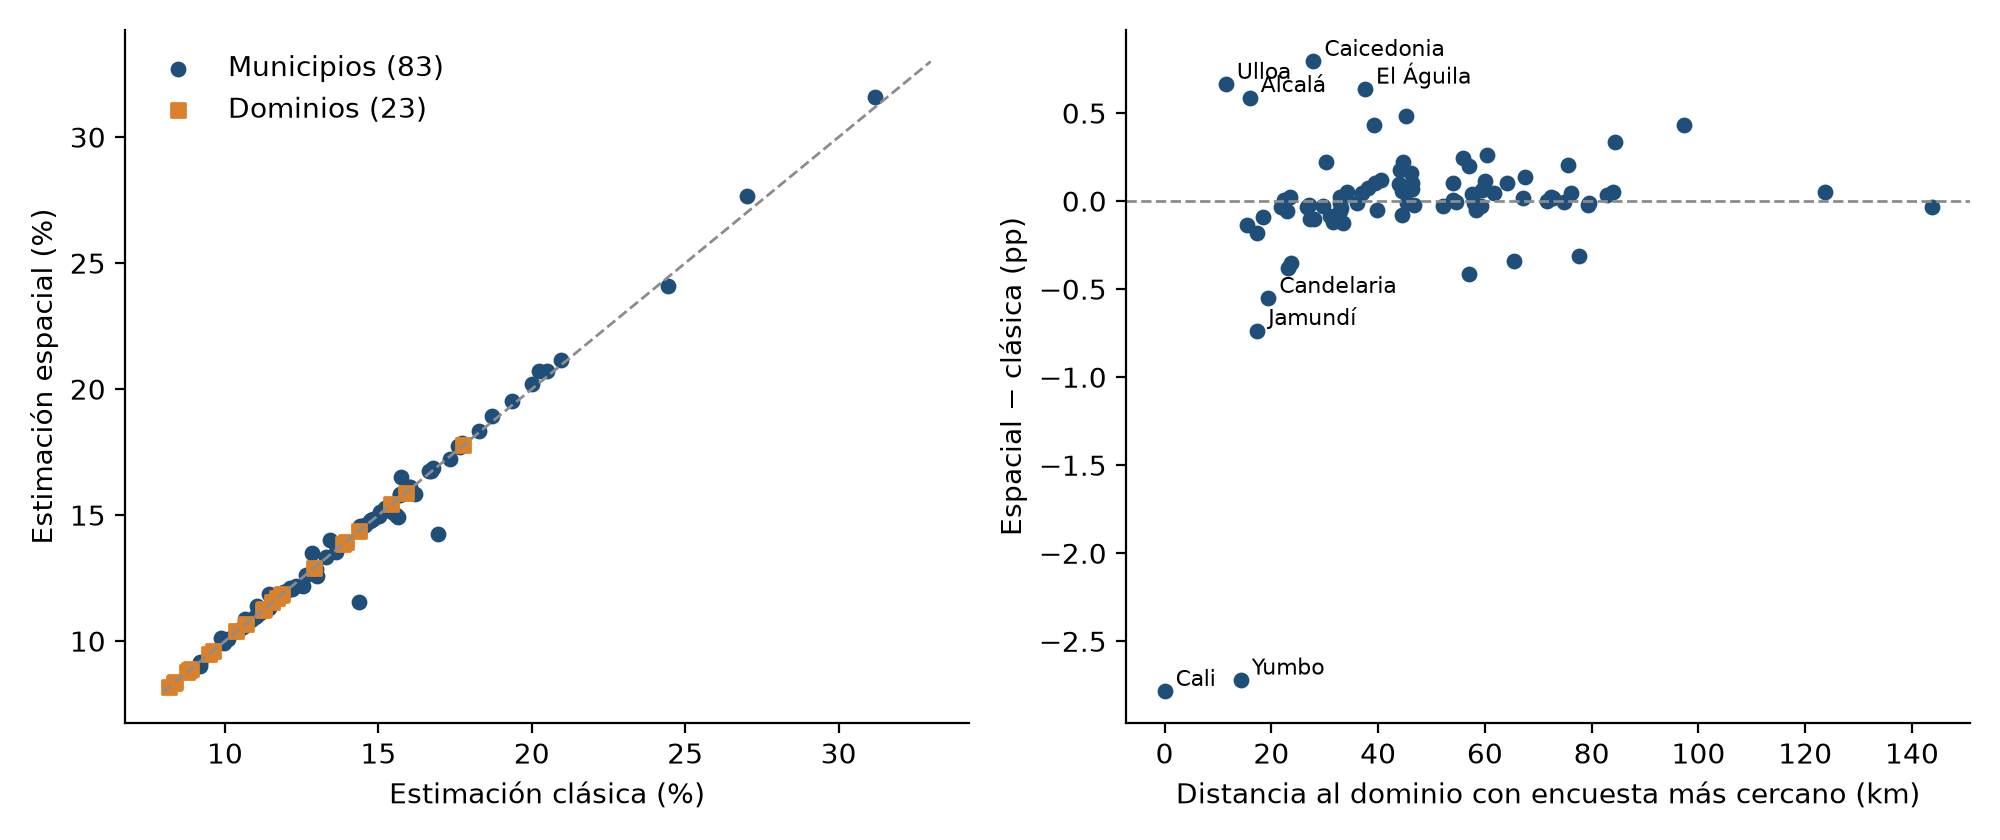
\includegraphics[width=\linewidth]{img/res_espacial_estimaciones.png}
\caption{Izquierda: estimación clásica frente a espacial en los 23 dominios (EBLUP y SEBLUP) y en los 83 municipios (sintética y espacial). Derecha: diferencia en los municipios según la distancia al dominio con encuesta más cercano; se nombran los que difieren más de 0.5 puntos porcentuales. Fuente: tabla de estimaciones de los municipios objetivo del modelo espacial y cálculo propio de los dominios.}
\label{fig:res_espacial_estimaciones}
\end{figure}

En la validación dejar-un-dominio-fuera con las covariables fijas (Tabla~\ref{tab:res_validacion_espacial} del Apéndice~\ref{app:resultados}), el predictor espacial del escenario de referencia tiene la menor RMSE: 2.35, frente a 2.48 de la estimación sintética espacial, 2.52 de la sintética clásica y 2.77 del modelo de solo intercepto, con habilidad de 0.28. La ventaja no se repite en los otros escenarios: con 5 vecinos sube a 2.59 y con distancia inversa a 2.60 y 2.86, este último con habilidad negativa. Con 23 dominios y covariables fijas, estas diferencias se leen como orden de magnitud y no cambian la conclusión del LRT.

%--------------------------------------------------------------------------------------
\section{Estimación en los municipios sin cobertura muestral}
\label{sec:res_sin_muestra}

La Figura~\ref{fig:res_rangos} compara la tasa de homicidios de los municipios objetivo con el rango de los dominios, que va de 4.06 (Tunja) a 71.96 (Quibdó) homicidios por cada 100,000 habitantes. En los municipios va de 0 a 221.47, con mediana 42.67. Tres municipios quedan por debajo del rango (Ginebra, Puracé y Silvia, sin homicidios en 2018) y 18 por encima, de modo que 21 de los 83 son extrapolación (Ecuación~\ref{eq:hnew}). Con una sola covariable no puede haber combinaciones atípicas: el estado de los otros 62 es «dentro del rango».

\begin{figure}[!htbp]
\centering
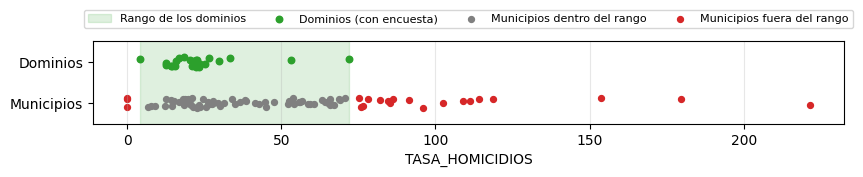
\includegraphics[width=\linewidth]{img/fh_rangos_covariables.png}
\caption{Tasa de homicidios de los 23 dominios y de los 83 municipios objetivo; la franja es el rango de los dominios. Fuente: tabla de rangos de covariables del Fay-Herriot clásico.}
\label{fig:res_rangos}
\end{figure}

La Tabla~\ref{tab:res_extrapolacion} resume las estimaciones sintéticas según su estado. En los 21 municipios que extrapolan, la parte de la estimación que viene de salirse del rango tiene mediana de 1.4 puntos porcentuales y máximo de 14.84, en Corinto, cuya estimación de 31.17~\% sería 16.33~\% con la tasa de homicidios recortada al máximo de los dominios. Diez municipios tienen una estimación mayor que 17.81~\%, la directa más alta de los dominios. Al retirar un dominio a la vez, la estimación de los que extrapolan se mueve en una franja mediana de 4.30 puntos porcentuales, frente a 0.79 en los que están dentro del rango (Figura~\ref{fig:app_sensibilidad_extrapolacion}).

\begin{table}[!htbp]
\centering
\small
\caption{Estimación sintética del benchmark en los 83 municipios, antes del benchmarking, según el estado de extrapolación. Tasas y RMSE en puntos porcentuales; CV en \%. Aporte: parte de la estimación que viene de salirse del rango.}
\label{tab:res_extrapolacion}
\begin{adjustbox}{max width=\linewidth}
\begin{tabular}{l r r r r r r}
\toprule
Estado y clase de CV & Municipios & Tasa media & Tasa máxima & CV medio & RMSE medio & Aporte medio \\
\midrule
Dentro del rango, aceptable & 33 & 14.36 & 16.19 & 18.48 & 2.65 & 0.00 \\
Dentro del rango, no confiable & 29 & 11.13 & 11.96 & 21.79 & 2.42 & 0.00 \\
Fuera del rango, aceptable & 15 & 18.36 & 20.96 & 18.85 & 3.47 & 2.03 \\
Fuera del rango, no confiable & 6 & 18.37 & 31.17 & 25.22 & 4.42 & 5.81 \\
\bottomrule
\end{tabular}
\end{adjustbox}
\end{table}

Ningún municipio queda confiable: el CV de la estimación sintética va de 18.07~\% a 27.71~\%, porque su ECM incluye $\hat{\sigma}_u^2 = 5.529$ completo (Ecuación~\ref{eq:var_sintetica}). El CV no distingue a los que extrapolan: su CV medio es 20.7~\% frente a 20.0~\% de los que no, aunque su RMSE medio es 1.5 veces mayor (3.74 frente a 2.54), porque la tasa estimada también sube y el cociente casi no cambia. Los CV más altos corresponden a las tasas más bajas, no a las estimaciones más dudosas: Ginebra, Puracé y Silvia, con tasa de 9.19~\%, igual al intercepto, tienen CV de 27.71~\%. Por eso la calidad reportada agrega la mención «condicional al modelo» a todos los municipios y «extrapolado (fuera del rango)» a los 21 que extrapolan. Las estimaciones de cada municipio con ambos modelos están en el Apéndice~\ref{app:municipios}.

%--------------------------------------------------------------------------------------
\section{Benchmarking y consolidación de las estimaciones}
\label{sec:res_benchmarking}

La Tabla~\ref{tab:res_benchmarking} presenta los dos niveles del benchmarking. En el nivel 1, el agregado de los 23 EBLUP ponderado por la PEA expandida es 10.8368~\% y la referencia es 10.8340~\%; el factor $\lambda_1 = 0.9997$ baja cada EBLUP entre 0.002 y 0.005 puntos porcentuales y no cambia ninguna clase. En el nivel 2, Cali y Yumbo, ponderados por su población de 15 años y más, suman 14.47~\%, mientras que el EBLUP ajustado de Cali A.M. es 11.69~\%: el factor $\lambda_D = 0.808$ los baja casi un 20~\%. La diferencia no viene de la forma de agregar las covariables: la brecha entre $\bar{\mathbf{x}}_D^\top\hat{\boldsymbol{\beta}}$ y el promedio ponderado de los sintéticos municipales es $-0.004$ puntos porcentuales. Viene de que Cali A.M. tiene una tasa de homicidios alta (el sintético del dominio es 14.48~\%) y una tasa directa mucho menor que la que anticipa esa covariable.

\begin{table}[!htbp]
\centering
\small
\caption{Benchmarking en dos niveles (Ecuaciones~\ref{eq:benchmarking} y~\ref{eq:rmse_bm}). Tasas en \%; CV en \% antes y después del ajuste.}
\label{tab:res_benchmarking}
\begin{tabularx}{\linewidth}{>{\raggedright\arraybackslash}X r r r r}
\toprule
Nivel y unidad & Antes & Referencia o después & $\lambda$ & CV antes y después \\
\midrule
Nivel 1: agregado de los 23 dominios & 10.84 & 10.83 & 0.9997 & sin cambio de clase \\
Nivel 2: agregado de Cali y Yumbo & 14.47 & 11.69 & 0.8077 & no aplica \\
\quad Cali & 14.36 & 11.60 & 0.8077 & 18.20 y 29.96 \\
\quad Yumbo & 16.96 & 13.70 & 0.8077 & 18.32 y 30.03 \\
\bottomrule
\end{tabularx}
\end{table}

Todas las verificaciones de la etapa pasaron: después del ajuste, el agregado reproduce la referencia con diferencias del orden de $10^{-15}$, las razones entre estimaciones se conservan, las tasas quedan en $[0, 100]$ y la comprobación sobre la tabla final redondeada también se cumple. El factor del nivel 2 supera el aviso de $|\lambda - 1| > 0.20$ por muy poco (0.192) y no lo activa, pero su efecto en la incertidumbre es grande: el sesgo $(\lambda - 1)\hat{\theta}$ del ajuste entra en la RMSE de la Ecuación~\ref{eq:rmse_bm} y el CV de Cali y Yumbo pasa de cerca de 18~\% a 30~\%, de modo que ambos quedan como no confiables.

La tabla final tiene 106 filas: los 23 dominios con el EBLUP ajustado, todos confiables (CV entre 2.01~\% y 3.20~\%), y los 83 municipios. La Tabla~\ref{tab:res_calidad} cuenta la calidad reportada de los municipios. En el Valle del Cauca la mitad de los municipios queda como aceptable dentro del rango (21 de 42); en el Cauca, 11 de 41. Frente a la Tabla~\ref{tab:res_extrapolacion}, Cali pasa de aceptable a no confiable y Yumbo, de aceptable extrapolado a no confiable extrapolado.

\begin{table}[!htbp]
\centering
\small
\caption{Calidad reportada de los 83 municipios en la tabla final, tras el benchmarking.}
\label{tab:res_calidad}
\begin{tabular}{l r r r}
\toprule
Calidad reportada & Cauca & Valle del Cauca & Total \\
\midrule
Aceptable, condicional al modelo & 11 & 21 & 32 \\
No confiable, condicional al modelo & 17 & 13 & 30 \\
Aceptable, condicional al modelo, extrapolado & 9 & 5 & 14 \\
No confiable, condicional al modelo, extrapolado & 4 & 3 & 7 \\
\midrule
Total & 41 & 42 & 83 \\
\bottomrule
\end{tabular}
\end{table}

%--------------------------------------------------------------------------------------
\section{Distribución y patrones espaciales de las estimaciones}
\label{sec:res_patrones}

La Figura~\ref{fig:res_mapa_municipios} muestra las 83 estimaciones finales, su calidad reportada y el efecto espacial. La tasa estimada va de 9.19~\% a 31.17~\%, con mediana de 13.29~\%. Los dos departamentos tienen promedios casi iguales (14.16~\% en el Cauca y 14.18~\% en el Valle del Cauca), pero el Cauca tiene más dispersión (desviación de 4.48 frente a 3.35) y más municipios que extrapolan (13 de 41 frente a 8 de 42). Las tasas más altas forman dos grupos: el norte del Cauca, con Corinto (31.17~\%), Puerto Tejada (24.46~\%), Guachené, Caloto y Villa Rica, y el norte del Valle, con El Águila (27.02~\%), Argelia, Ansermanuevo y Toro. Al sur del Cauca, Argelia (20.96~\%) y Patía (20.50~\%) también quedan altos. Todos esos municipios están entre los que extrapolan.

\begin{figure}[!htbp]
\centering
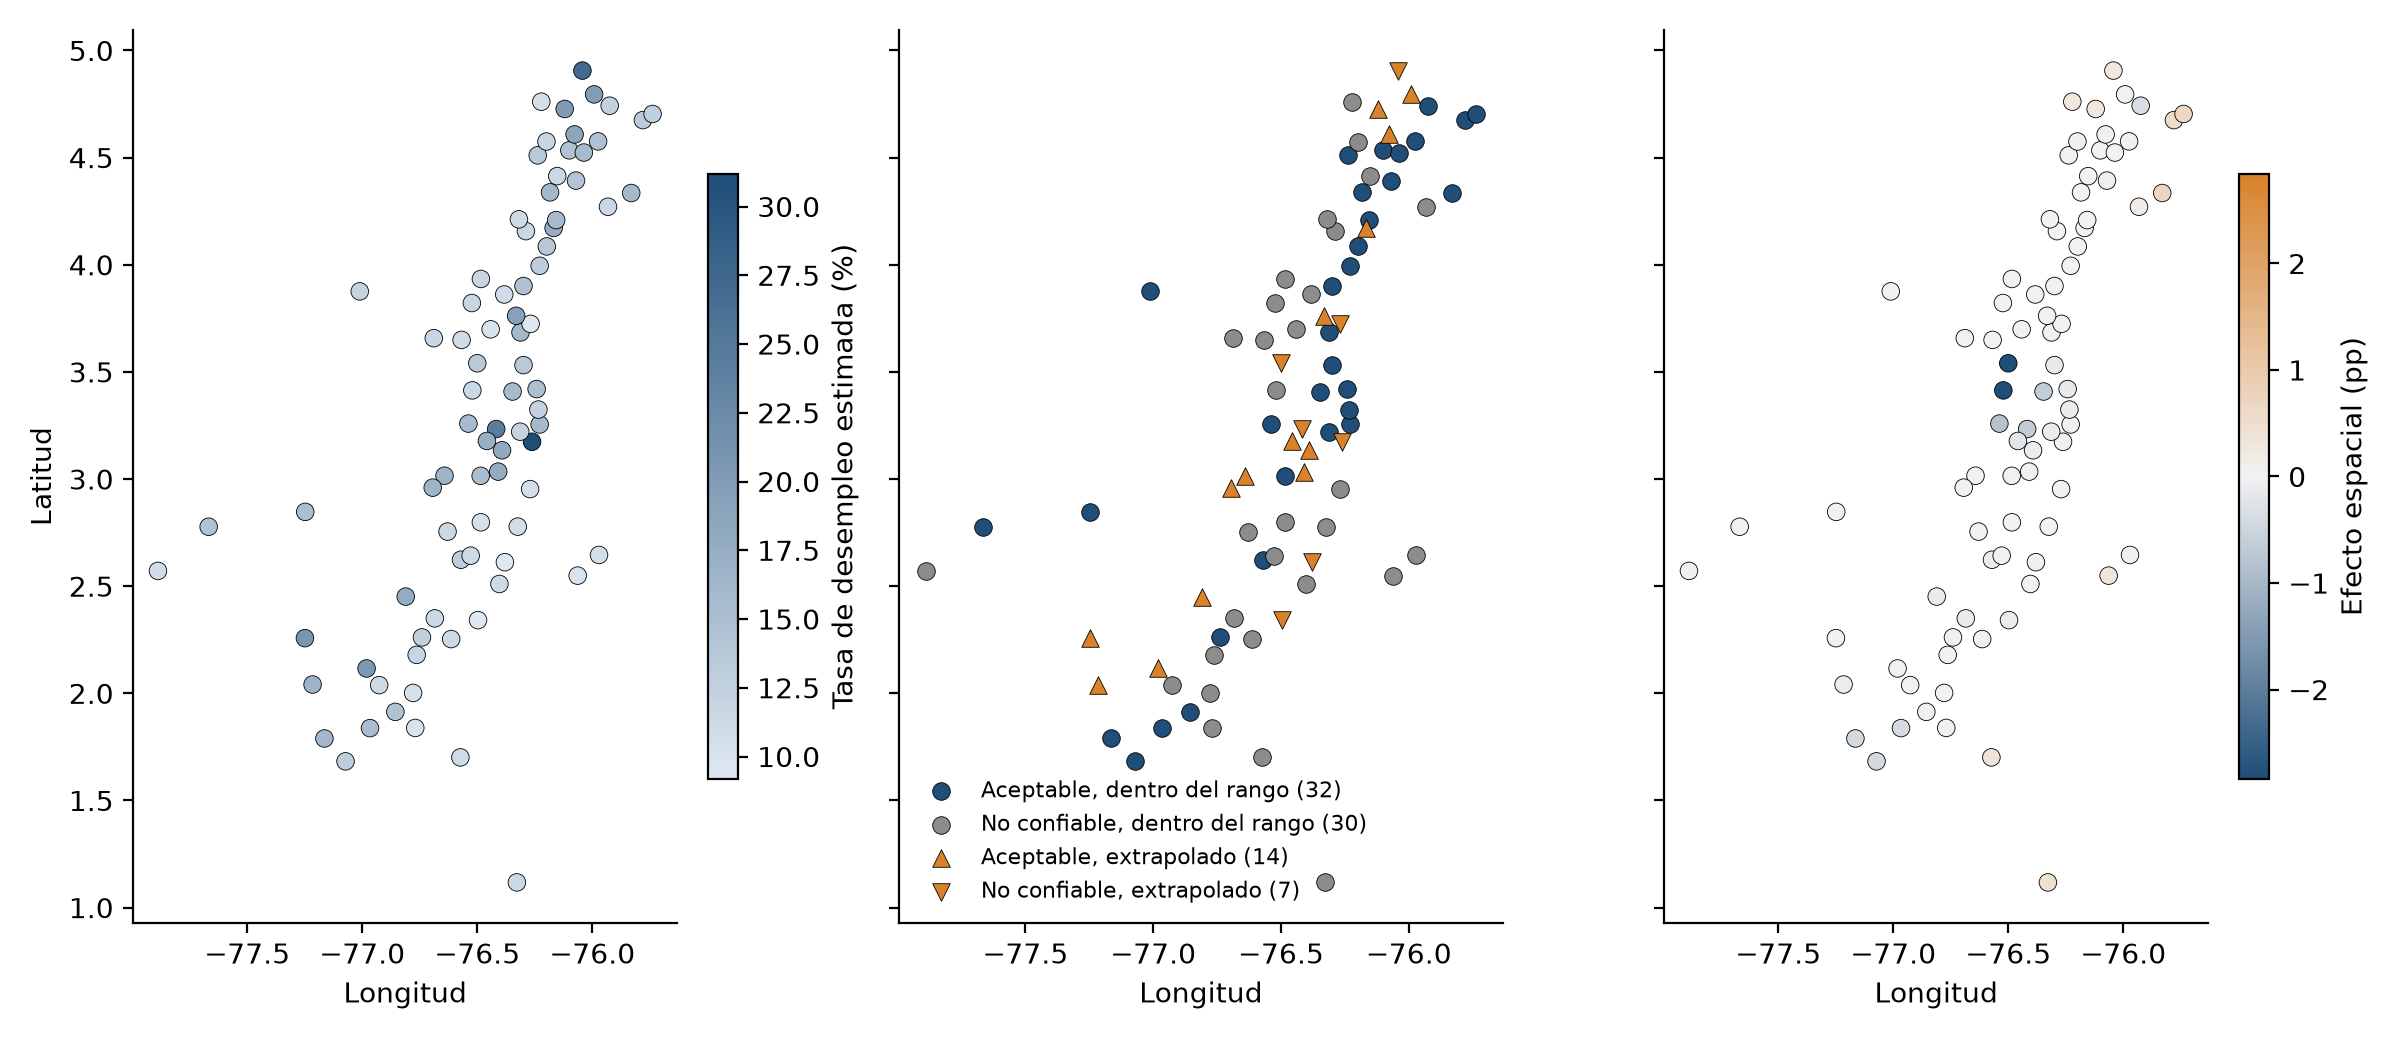
\includegraphics[width=\linewidth]{img/res_mapa_municipios.png}
\caption{Municipios objetivo ubicados en su cabecera. Izquierda: tasa de desempleo estimada en la tabla final. Centro: clase de CV y estado de extrapolación. Derecha: efecto espacial del escenario de referencia (estimación espacial menos sintética). Fuente: tabla final consolidada y tabla de estimaciones de los municipios objetivo del modelo espacial.}
\label{fig:res_mapa_municipios}
\end{figure}

Las estimaciones finales tienen autocorrelación espacial positiva: con 3 vecinos, el I de Moran es 0.265 ($E[I] = -0.012$; $p = 0.001$ con \num{9999} permutaciones). El patrón viene de la covariable: la tasa de homicidios de los mismos 83 municipios, con la misma matriz, tiene $I = 0.256$ y el mismo $p$, y la estimación sin benchmarking da prácticamente el mismo valor (0.256), porque es una función lineal de esa tasa. El efecto espacial no agrega un patrón propio: es menor que 0.5 puntos porcentuales en 75 de los 83 municipios y solo es grande en Cali y Yumbo, por el efecto de su dominio. Por eso, los grupos del mapa reflejan dónde hubo más homicidios en 2018, no un patrón del desempleo observado en esos municipios.

%--------------------------------------------------------------------------------------
\section{Correspondencia entre etapas y objetivos}
\label{sec:res_objetivos}

La Tabla~\ref{tab:res_objetivos} reúne, para cada objetivo, la evidencia principal de este capítulo, en el orden de la Tabla~\ref{tab:met_objetivos}.

\begin{table}[!htbp]
\centering
\small
\caption{Evidencia de Resultados por objetivo. OG: objetivo general; OE: objetivo específico.}
\label{tab:res_objetivos}
\begin{tabularx}{\linewidth}{>{\raggedright\arraybackslash}p{1.4cm} >{\raggedright\arraybackslash}X >{\raggedright\arraybackslash}p{3.4cm}}
\toprule
Objetivo & Resultado principal & Evidencia \\
\midrule
OG & Procedimiento completo y reproducible de 16 etapas; 23 dominios con directa confiable y validada contra el DANE; 83 municipios con estimación, ECM, estado de extrapolación y calidad reportada & Tablas~\ref{tab:res_directa}, \ref{tab:res_calidad}; Apéndice~\ref{app:municipios} \\
OE1 & Benchmark EC3; ocho especificaciones espaciales sin evidencia de $\rho \neq 0$ ($p \geq 0.221$) ni Moran significativo; estimaciones prácticamente iguales en dominios y con diferencia absoluta media de 0.22 puntos en municipios & Tablas~\ref{tab:res_espacial}, \ref{tab:res_moran}, \ref{tab:res_comparacion} \\
OE2 & Una covariable, la tasa de homicidios ($\hat{\beta} = 0.099$), asociada positivamente con la tasa; depende de Quibdó y el procedimiento completo estima peor que el modelo nulo (habilidad $-0.54$) & Tablas~\ref{tab:res_coeficientes}, \ref{tab:res_estabilidad}, \ref{tab:res_validacion} \\
OE3 & Tasas más altas en el norte del Cauca y el norte del Valle, todas extrapoladas; Moran de 0.265 que repite el de la tasa de homicidios; efecto espacial menor que 0.5 puntos en 75 de 83 & Figura~\ref{fig:res_mapa_municipios}; Sección~\ref{sec:res_patrones} \\
\bottomrule
\end{tabularx}
\end{table}
\FloatBarrier
